\documentclass[12pt]{article}
\usepackage[table]{xcolor}
\usepackage[shortlabels]{enumitem}
\usepackage{tabularx,xltabular}
\usepackage{graphicx}
\usepackage{hyperref}
\usepackage{verbatim}
\usepackage{geometry}
\usepackage{ulem}
\usepackage[official]{eurosym}
\usepackage{tikz}
\usetikzlibrary{arrows,backgrounds,calc,decorations.markings,patterns,3d}
\usepackage{pgfplots}
\pgfplotsset{compat = newest}
\usetikzlibrary{fit}
\newcommand\addvmargin[1]{
\usetikzlibrary{arrows}
\node[fit=(current bounding box),inner ysep=#1,inner xsep=0]{};}
\usepackage{cancel}
\usepackage{fontspec}
\usepackage{array}  
\geometry{a4paper, top=2cm, left=2cm, right=2cm, bottom=2cm, headsep=1cm}
\usepackage{tabu}
\usepackage{pst-node}
\usepackage{colortbl}
\usepackage{array}
\usepackage{german}
\setlength\parindent{0pt}
\newcolumntype{?}{!{\vrule width 1pt}}
\usepackage{makecell}
\renewcommand{\arraystretch}{2.5}
\usepackage{pbox}
\usepackage{amssymb}
\usepackage{amsmath}
\usepackage{booktabs}
\newcolumntype{L}[1]{>{\raggedright\let\newline\\\arraybackslash\hspace{0pt}}m{#1}}
\newcolumntype{C}[1]{>{\centering\let\newline\\\arraybackslash\hspace{0pt}}m{#1}}
\newcolumntype{R}[1]{>{\raggedleft\let\newline\\\arraybackslash\hspace{0pt}}m{#1}}
\begin{document}
\rightline{Datum: 12.06.2023}
\centerline{{\Large Tägliche Übungen}} 
\vspace{1cm}
\noindent \\


\begin{xltabular}{\textwidth}{|C{0.75cm}|X|C{0.75cm}|X|}
\arrayrulecolor{black}\hline
a)&$-2\cdot y+2-7+5\cdot y=1$
&
b)&$-8-1\cdot a+1+4\cdot a=11$
\\\hline
c)&$5\cdot x+1\cdot x+5-19=46$
&
d)&$-29-2\cdot b+12+5\cdot b=4$
\\\hline
\end{xltabular}
\vspace{0.5cm}
\noindent\tikzstyle{background grid}=[draw, black!30,step=.5cm]

\begin{tikzpicture}[show background grid]
\node[] at (0,0) {};
\node[] at (16,12) {};
\end{tikzpicture}
\\
\newpage
\rightline{Datum: 12.06.2023}
\centerline{{\large Lösungen Tägliche Übungen}} 
\vspace{0.5cm}

\begin{xltabular}{\textwidth}{|C{0.75cm}|X|}
\arrayrulecolor{black}\hline
a)&\begingroup\setlength{\jot}{-0.03cm}
\tikzstyle{background grid}=[draw, black!15,step=.5cm]
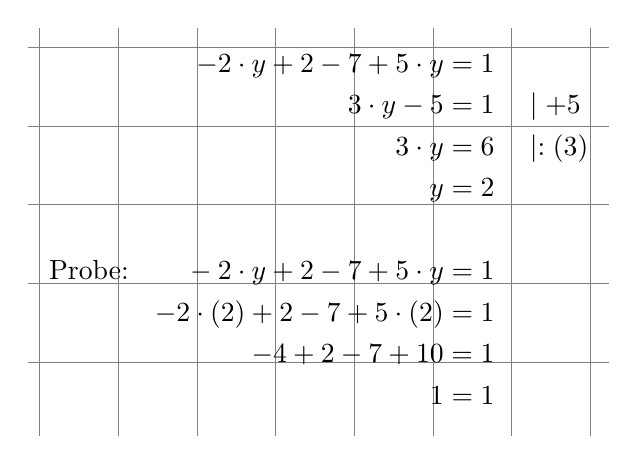
\begin{tikzpicture}[show background grid]
\node[below right] at (0,0.1) {
$\begin{aligned}
-2\cdot y+2-7+5\cdot y &=1& &  \\
3\cdot y - 5 &=1& & \mid + 5\\
3\cdot y &=6& & \mid :\left(3\right)\\
y &=2& & 
\\
\\
\mbox{Probe:}\qquad -2\cdot y+2-7+5\cdot y &=1& &  \\
-2\cdot \left(2\right)+2-7+5\cdot \left(2\right) &=1& &  \\
-4+2-7+10 &=1& &  \\
1 &=1& &  \\
\end{aligned}$};
\end{tikzpicture}
\endgroup
\\\hline
b)&\begingroup\setlength{\jot}{-0.03cm}
\tikzstyle{background grid}=[draw, black!15,step=.5cm]
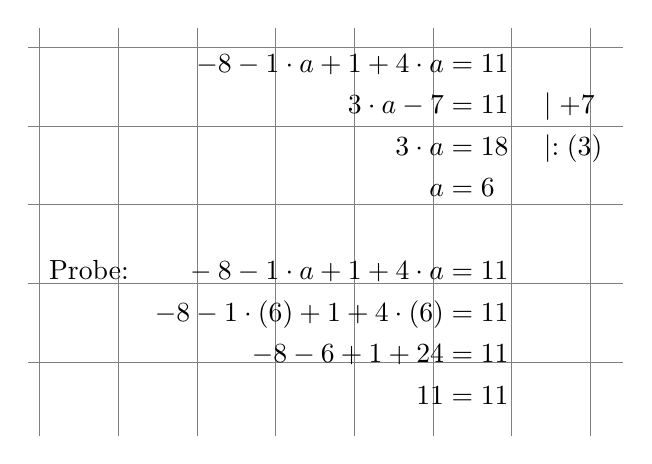
\begin{tikzpicture}[show background grid]
\node[below right] at (0,0.1) {
$\begin{aligned}
-8-1\cdot a+1+4\cdot a &=11& &  \\
3\cdot a - 7 &=11& & \mid + 7\\
3\cdot a &=18& & \mid :\left(3\right)\\
a &=6& & 
\\
\\
\mbox{Probe:}\qquad -8-1\cdot a+1+4\cdot a &=11& &  \\
-8-1\cdot \left(6\right)+1+4\cdot \left(6\right) &=11& &  \\
-8-6+1+24 &=11& &  \\
11 &=11& &  \\
\end{aligned}$};
\end{tikzpicture}
\endgroup
\\\hline
c)&\begingroup\setlength{\jot}{-0.03cm}
\tikzstyle{background grid}=[draw, black!15,step=.5cm]
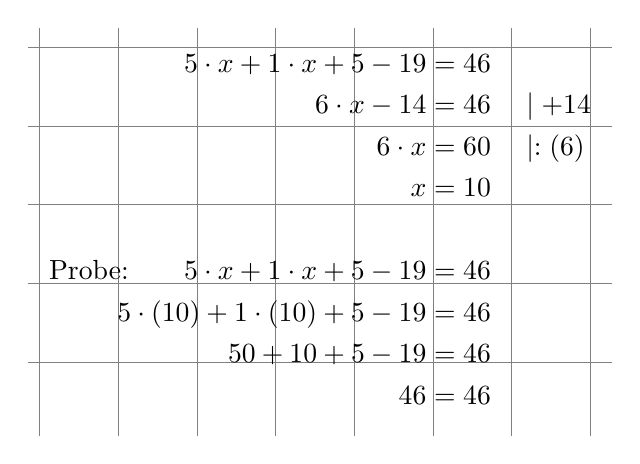
\begin{tikzpicture}[show background grid]
\node[below right] at (0,0.1) {
$\begin{aligned}
5\cdot x+1\cdot x+5-19 &=46& &  \\
6\cdot x - 14 &=46& & \mid + 14\\
6\cdot x &=60& & \mid :\left(6\right)\\
x &=10& & 
\\
\\
\mbox{Probe:}\qquad 5\cdot x+1\cdot x+5-19 &=46& &  \\
5\cdot \left(10\right)+1\cdot \left(10\right)+5-19 &=46& &  \\
50+10+5-19 &=46& &  \\
46 &=46& &  \\
\end{aligned}$};
\end{tikzpicture}
\endgroup
\\\hline
d)&\begingroup\setlength{\jot}{-0.03cm}
\tikzstyle{background grid}=[draw, black!15,step=.5cm]
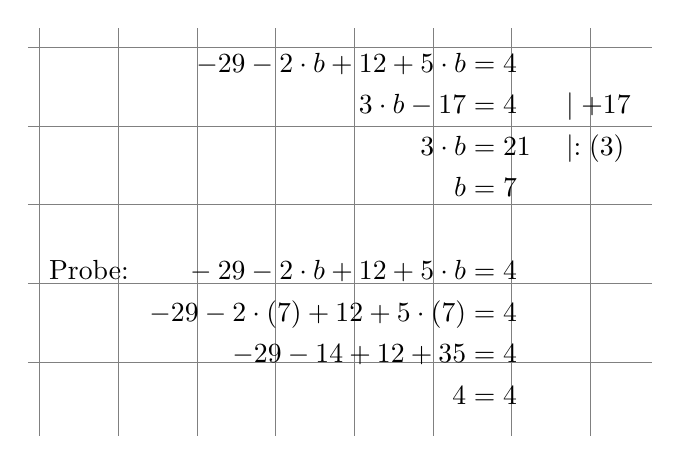
\begin{tikzpicture}[show background grid]
\node[below right] at (0,0.1) {
$\begin{aligned}
-29-2\cdot b+12+5\cdot b &=4& &  \\
3\cdot b - 17 &=4& & \mid + 17\\
3\cdot b &=21& & \mid :\left(3\right)\\
b &=7& & 
\\
\\
\mbox{Probe:}\qquad -29-2\cdot b+12+5\cdot b &=4& &  \\
-29-2\cdot \left(7\right)+12+5\cdot \left(7\right) &=4& &  \\
-29-14+12+35 &=4& &  \\
4 &=4& &  \\
\end{aligned}$};
\end{tikzpicture}
\endgroup
\\\hline
\end{xltabular}
\vspace{0.5cm}
\end{document}